% TEMPLATE for Usenix papers, specifically to meet requirements of
%  USENIX '05
% originally a template for producing IEEE-format articles using LaTeX.
%   written by Matthew Ward, CS Department, Worcester Polytechnic Institute.
% adapted by David Beazley for his excellent SWIG paper in Proceedings,
%   Tcl 96
% turned into a smartass generic template by De Clarke, with thanks to
%   both the above pioneers
% use at your own risk.  Complaints to /dev/null.
% make it two column with no page numbering, default is 10 point

% Munged by Fred Douglis <douglis@research.att.com> 10/97 to separate
% the .sty file from the LaTeX source template, so that people can
% more easily include the .sty file into an existing document.  Also
% changed to more closely follow the style guidelines as represented
% by the Word sample file. 

% Note that since 2010, USENIX does not require endnotes. If you want
% foot of page notes, don't include the endnotes package in the 
% usepackage command, below.

% This version uses the latex2e styles, not the very ancient 2.09 stuff.
\documentclass[letterpaper,twocolumn,10pt]{article}
\usepackage{usenix,epsfig,endnotes}
\begin{document}

%don't want date printed
\date{}

%make title bold and 14 pt font (Latex default is non-bold, 16 pt)
\title{\Large \bf Learning Malware Behavior: A Bottom-Up Approach}

%for single author (just remove % characters)
\author{
{\rm Daniel Byrne}\\
Michigan Technological University
\and
{\rm Jinxin Fang}\\
Michigan Technological University
% copy the following lines to add more authors
\and
{\rm Bochao Li}\\
Michigan Technological University
\and
{\rm Jiancheng Li}\\
Michigan Technological University
\and
{\rm Nilufer Onder}\\
Michigan Technological University
} % end author

\maketitle

% Use the following at camera-ready time to suppress page numbers.
% Comment it out when you first submit the paper for review.
\thispagestyle{empty}


\subsection*{Abstract}
Malware detection is a difficult problem in industry and government. We cannot create signatures for unknown malware behavior, but we can measure when a host may be executing a malicious piece of software~\cite{idika2007survey}. In this work we propose to use architecture level information to learn what constitutes normal program behavior. We use metrics such as, instruction and data reuse, branch direction, memory accesses, and dependencies, since they provide an intimate description of a program’s execution. We measure these using Intel PIN tool ~\cite{luk2005pin} and build a dataset from malware samples executed. We then build an artificial neural network from the newly released TensorFlow by Google ~\cite{abadi2016tensorflow} to classify programs as malicious or normal. With 61 reference normal programs from SPEC CPU benchmarks~\cite{spec} and 113 pieces malware from theZoo~\cite{thezoo}, we obtain 86\% accuracy. These results provide a promising starting point for using architecture level information as a robust basis for detection in a constantly evolving landscape of malware. We also promote this technique for detection of zero-day exploits and offering security experts the ability to discover malicious programs in a shorter period of time.

\section{Introduction}

From the over 1.4 million submissions to the malware database VirusTotal~\cite{virustotal} made everyday, there are nearly 400,000 distinct pieces detected. What we do not know is how many of those 1.4 million submissions are unknown pieces of malware, yet to be discovered by traditional methods. To complicate matters, malware developers are constantly evolving source code in order to avoid detection mechanisms~\cite{anderson2014automating}. 

In industry and government, the process of detecting malware is a difficult problem for security experts when encountered with a piece of unknown software that may be targeted at their specific site~\cite{anderson2014automating}. This is because often times, targeted malware does not leave behind the traditional fingerprints that prior works have relied on for detection.

Currently, there exist two main techniques for malware classification, signature based and behavior based. Signature based techniques look for known properties of malware, these come in the form of hashes or YARA rules~\cite{yara}. For known malware, these rules work well. But the problem is that they cannot capture the entire domain of malicious behavior, nor can they detect zero-day exploits~\cite{idika2007survey}. 

Behavior based techniques require execution of the suspected malware in order to analyze the artifacts created during execution ~\cite{idika2007survey}. It requires us to train the detection mechanism to know what is normal behavior and what behavior should be considered malicious. The key challenge in behavior-based detection is looking for which artifacts of program execution constitute normal and malicious behavior. 

Artifacts are typically found throughout the filesystem and in the system registry (or configuration files). Much prior work has focused around selecting the proper features of artifacts in order to improve detection and classification ~\cite{mohaisen2013unveiling}, but these have all relied on malware leaving its fingerprint on the operating system. Our insight is to use information at the architecture level to detect malware. This aids security researchers in discovering new pieces of malware before there exists a known signature and can significantly reduce the amount of time between malware intrusion and detection.


\section{Background and Related Work}
Recent research results suggest that static malware analysis alone may no longer be adequate to identify emerging types of malware~\cite{moser2007limits}. Mohaisen and Alrawi have developed several classifiers based on 65 features of artifacts found after malware execution. They achieve good accuracy (about 95\%), but have only verified these results with against a well known malware family, Zeus~\cite{mohaisen2013unveiling}.

Program similarity has been used to evaluate the effectiveness of CPU benchmarks by ensuring that programs selected have weak locality and weak similarity scores, since the focus of benchmarks should cover a broad spectrum of application types~\cite{phansalkar2007analysis}.

In addition, it has been shown that applications who score similar, will have similar performance and behavior in the architecture ~\cite{hoste2006performance}. This supports the idea that locality metrics and other instruction information can create a representative feature vector for a given class of malware.

Locality metrics have been used to improve cache performance~\cite{hu2016kinetic} and offer a candid look at how a program executes~\cite{xiang2013hotl}. Prior work has combined these locality metrics with other architecture metrics in order to measure similarity throughout a set of programs~\cite{phansalkar2005measuring}. 

We extend the characterization methodology set forth in~\cite{phansalkar2005measuring} in order to build our classifier by gathering the same set of metrics on malware. We then build a neural network to classify programs into two classes: normal or malware.

\subsection{Architecture Background}

A dynamic instruction trace can provide a key insight into the execution of a program. Branches are instructions that when a condition is satisfied, they will jump to another section of code. Typically branches make up on the order of 5-30\% of a program’s instructions~\cite{bird2007performance}. Not only the frequency, but the direction of these branches is important in determining the control flow of the program. A back-taken branch, makes the new program counter (PC) less than the previous. This is highly correlated with repeating a loop since previous instructions will be executed again. A forward-taken branch is important since we may be moving on to different sections of the code or into libraries.

Memory instruction are typically load and store operations. They tend to make up almost 40\% of all the program’s instructions ~\cite{bird2007performance}. Arithmetic instructions: add, subtract, multiply, divide, and shifts, are important in determining how much computation a program is performing. Measuring the ratio of memory to arithmetic helps us know if a program relies on memory or compute instructions~\cite{phansalkar2005measuring}. 

In addition, we measure the amount of locality in the program and the dependencies. Program locality has two types: spatial and temporal~\cite{ding2003predicting}. Spatial locality is best defined as how close in space a program’s instructions or data is reused. Temporal locality is defined by how close in time a program’s instructions or data is reused. Next, we measure only true dependencies, that is read-after-write (RAW) dependencies. 

Finally, we measure the size of a basic block, a basic basic block is a sequence of instructions that have a single point of entry and single point of exit. They are typically 5-20 instructions in length. 

\subsection{Artificial Neural Network}
Artificial neural networks are computer program that learning from a large number of collections~\cite{hinton2006fast}. It is loosely based on the way brain solves problems. All the neurons are created and connected with others, the connections can be enforcing or inhibitory on the activation state. The network is asked to repeatedly solve the problems, each time strengthening the connections. Each neuron has its own summation function to combine all the input values before propagate to other neurons. The neurons’ function could be a limiting function or a threshold function. 

We use TensorFlow~\cite{abadi2016tensorflow}, an open source software library, developed by Google, to build our model. TensorFlow allows us to preprocess our data and build the deep neural network through its API.

As preliminary investigation, we trained a model using dataset of 61 SPEC CPU programs from years 1989 to 2000. We classified the programs as integer-based or float-based, with an accuracy of 94\%. This gives us confidence in our model for detecting malware specific behavior using the proposed metrics.

\section{Malware Detection}
\subsection{System Overview}

\begin{figure}[!htb]
\centering
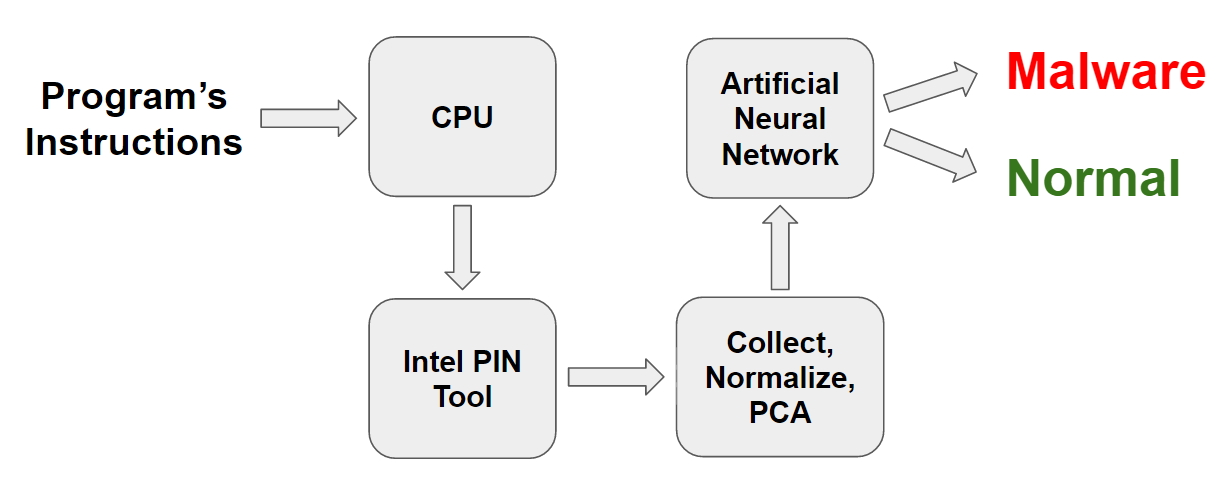
\includegraphics[width=0.7\textwidth]{images/system_architecture.png}
\caption{System architecture block diagram.}
\label{fig:sys}
\end{figure}

The idea of this project is to detect malware based on their behavior at the hardware level. The system architecture is shown in Figure~\ref{fig:sys}. First, when a program is running, it generates machine-level instructions, which will be captured and analyzed dynamically by the Intel Pintool program. Then, we will process and feed the data into a pre-trained ANN, and produce a prediction for the program class: normal or malware.

\subsection{Collecting Metrics}

A Pintool is a program that used to perform program analysis dynamically. It is developed with Pin, a software system that performs run-time binary instrumentation of applications ~\cite{luk2005pin}.To get the features described above, we measured the following: 


\begin{itemize}
\item Memory accesses
\item Percentage of computation instructions
\item Basic block size
\item Branches taken, including forward and backward branches taken
\item Dependency distance with distance 2, 4, 8, 16, 32 and greater than 32
\item Data temporal locality over window sizes: 16, 64, 256 and 4096
\item Data spatial locality over window sizes: 16, 64, 256 and 4096
\item Instruction temporal locality over window sizes: 16, 64, 256 and 4096
\item Instruction spatial locality over window sizes: 16, 64, 256 and 4096
\end{itemize}

For normal program data we build off of previous work collected in ~\cite{phansalkar2005measuring} and then combine with our data.

To gather sample data of malware behaviors, we used a free and open malware database, theZoo~\cite{thezoo}. From the repository, we downloaded the binaries of 133 different types of win32 malware. For safe execution, we used a Windows 7 virtual machine with no internet access. We then ran the malware under our Pintool to obtain the behavior sample for each malware.

There were two difficulties encountered while collecting data. First some malware created a child processes during execution. Since our Pintool program was only attached the original malware process, any new processes created by the malware were not captured. Second, some malware would stall, waiting for some resource, which makes termination difficult. By setting the termination goal of the Pintool program based on different types of malware, we successfully collected 113 data samples from different malware. 

\subsection{Principle Component Analysis} 

In our analysis, we measured 29 metrics based on~\cite{hoste2006performance} as we have described. Dimensionality reduction is necessary to remove noise and succinctly describe the data~\cite{yu2003feature}, therefore we employ Principal Component Analysis~\cite{jolliffe2002principal}. Principle component analysis (PCA) is a common statistical technique, which significantly decreases the number of features by converting the original set of features to a set of linearly uncorrelated principal components (PCs). Each PC is a linear combination of the original features. In our project, after obtaining the data samples, we first normalized all the features, and then applied PCA to the data using Weka~\cite{hall2009weka}, which then output five PCs that covered 95\% of the original data variance.

\subsection{Building Artificial Neural Network using TensorFlow}

\begin{figure}[h!t]
\centering
\includegraphics[width=0.9\textwidth]{images/ANN.png}
\caption{Artificial neural network with three hidden layers.}
\label{fig:ann}
\end{figure}

Once we separate the data into train and test tests. We create an artificial neural network(ANN) classifier to build up the model. The ANN we used for this project is inherited from the Iris flower classification project~\cite{iris}, which has three hidden layers with 10, 20, 10 nodes on the layers, shown in Figure~\ref{fig:ann}. 

\subsection{Result and Discussion} 

\begin{figure}[!ht]
\centering
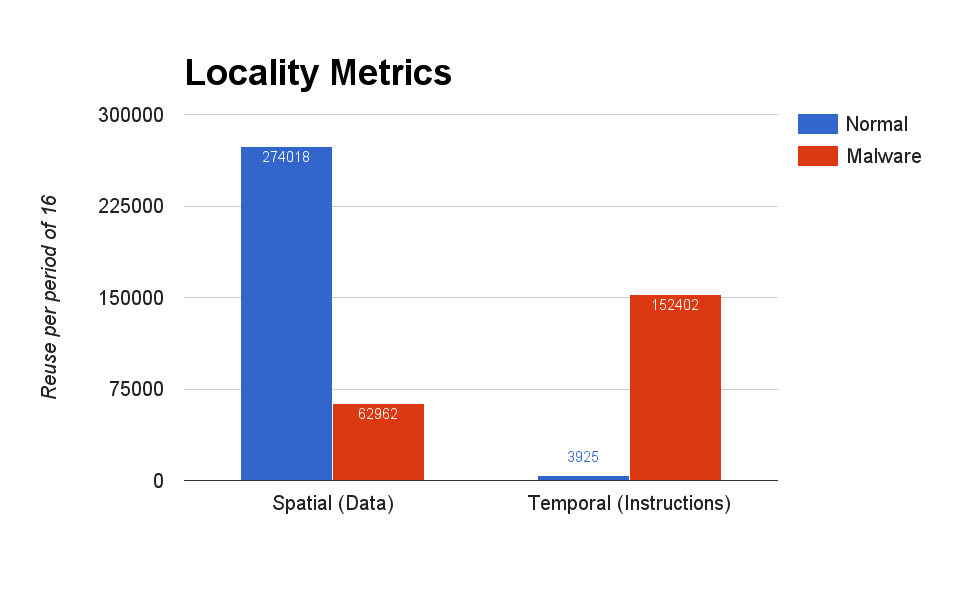
\includegraphics[width=0.85\textwidth]{images/locality.png}
\caption{Comparison of locality metrics between normal and malware programs.}
\label{fig:locality}
\end{figure}

We select a subset of features from each principle component (in order of variance explained) to give the reader an idea of what malware execution looks like at the architecture level. 

\begin{itemize}
\item \textbf{Average Temporal Instruction Locality}

It has been observed that the malware samples run same parts of code often due to waiting on user input (ie. credit card information or password) or communication from a server. This is supported by the large amount of temporal instruction locality that we measured. In the Figure~\ref{fig:locality}, we see that there is a much high rate of instruction reuse in a window of 16 distinct instructions. In fact, on average malware samples reuse 148477 more instructions. 

\item \textbf{Average Temporal Data Locality}

Our results suggest malware access a wider range of data throughout its execution. This is due to the fact that normal program involves orders of magnitude more accesses to common data structures when performing useful operation. Unlike normal programs, malware does not constantly access its data structures to perform useful tasks since it is often just waiting to exfiltrate personal information.

\item \textbf{Branch behavior}
 
As a whole, we observe that malware has about 6.5\% less branches that our normal program set. While this is not a key factor in determining program behavior, it promotes the idea that the instruction makeup of malware is fundamentally different than that of a normal program.  

As further evidence of a large portion of a malware sample being composed of loops, is the number of branches that are back-taken. On average we see that malware samples have 21\% more back-taken branches than our normal program set. This directly supports what has been observed in measuring the average temporal instruction locality metric.

\item \textbf{Instruction Mix}

The compute to memory instruction ratio tells us that malware is heavily memory bound, rarely performing computation instructions. This suggests that the malware often is gathering data or attempting to access system and personal information stored in RAM.

\item \textbf{Basic Block size} 

There is not a significant enough difference in basic block size to distinguish malware from normal program execution. While on average basic blocks are smaller in malware samples, they do not play a key role in detection. In future work, this metric may be removed.

\end{itemize}

Our TensorFlow neural network resulted in 86\% accuracy. This gives us reasonable confidence in determining if a given program execution is malicious or not. Of course, building a larger dataset will give us more confidence towards practical usage since the cost of false positives (programs that are identified as malicious but are really just normal), is high. Reducing the false positive rate is left for future work.

% you can also use the wonderful epsfig package...
\begin{figure}[t]
\begin{center}
\begin{picture}(300,150)(0,200)
\put(-15,-30){\special{psfile = ratio.ps hscale = 50 vscale = 50}}
\end{picture}\\
\end{center}
\caption{Comparison of instruction metrics between normal and malware programs.}
\end{figure}



\section{Conclusion}

As of now, there has been little research done in using architecture level information to detect malware. We have successfully collected a significant amount of malware data samples and shown with reasonable accuracy (86\%) that malware can be classified using the data we collected. This supports the idea that malware does have some common instruction-level characteristics. We present this work as a motivation to improve the effective and efficiency of the current malware protection systems. Especially in determining if an unknown piece of software is potential malware. 


As malware continues to grow in complexity, we need to shorten time between intrusion and detection. This reduces data loss for organizations and makes developing malware less attractive. But for now, as the forms of malware continue to evolve, architectural level information provides a robust set of metrics to confidently measure program behavior.


\bibliographystyle{acm}
\bibliography{paper}
\nocite{*}



\theendnotes

\end{document}







